\documentclass{article}
\usepackage{amsmath}
\usepackage[margin=0.5in]{geometry}
\usepackage{graphicx}
\usepackage{float}
\usepackage{caption}

\setlength{\parskip}{\baselineskip}%
\setlength{\parindent}{0pt}%

\title{STAT 788 - Homework 2}
\author{Daniel Hartig}


\begin{document}

\subsubsection*{Error definitions}

This is a greedy search of all possible features to find the best 'path' to a regression solution. First, all features are checked by regression against ridership. After choosing the one feature that yields the highest score, we then select a second feature to add to the regression in in the same way, and iteratively add more features.

Three separate accuracy metrics are used: summed absolute error as a percentage, mean absolute percentage error (MAPE), and system absolute percentage error. Given a length $n$ set of predicted ridership values, $\hat{y_i}$, and a set of true ridership values, $y_i$, summed absolute error by percentage is 
$$E_{sum} = 1 - \frac{\sum|\hat{y}_i-y_i|}{\sum y_i}.$$ The advantage of summed absolute error is that error in absolute number of riders is weighted evenly over the entire system, by dividing by the sum of all individual station errors by the sum of system ridership. By contrast, MAPE weights absolute error in the larger stations less significantly, since it divides by those station's larger ridership. MAPE is
$$E_{MAPE} = 1 - \frac{1}{n}\sum \frac{|\hat{y}_i-y_i|}{y_i}.$$ System error is 
$$E_{sys} = 1 - \frac{\left|\sum \hat{y}_i - \sum y_i\right|}{\sum y_i}.$$

Each feature is checked in six-way cross validation. Each of the six cities is used as the test set while the other five are used for the training set. The average over all six cross-validation runs for each metric is what is reported in the charts below. The average of the three metrics is used to select the best feature in each iteration.



\subsubsection*{Regression results}

For three regression types--Poisson with identity link, Linear Least Squares, and Linear Least Absolute Deviation (LAD)--we report the three metrics for the first 20 variables added this way. 

\begin{center}
\begin{tabular}{ c c c c c c c }
\hline
Regression Type&&Added Variable&Summed Station Error&MAPE&System Error \\
\hline
Poisson&1&15net\_hunits\_old&0.3131&-0.3266&0.6622\\
&2&60net\_university&0.3165&-0.1524&0.6371\\
&3&near\_hospitality&0.3593&-0.0848&0.6576\\
&4&parking&0.3653&-0.0024&0.6648\\
&5&near\_population&0.3750&0.0388&0.6934\\
&6&near\_family&0.3742&0.0477&0.6969\\
&7&near\_business&0.3770&0.0563&0.6929\\
&8&15net\_hospitality&0.3735&0.0646&0.6870\\
&9&15net\_finance&0.3782&0.0667&0.6962\\
&10&near\_hunits\_large&0.3794&0.0690&0.7141\\
&11&15net\_emp\_pay&0.3878&0.0492&0.7309\\
&12&15net\_university&0.3918&0.0594&0.7370\\
&13&near\_medical&0.3934&0.0650&0.7383\\
&14&near\_entertainment&0.3924&0.0732&0.7361\\
&15&near\_hunits\_vacant&0.3905&0.0834&0.7327\\
&16&30net\_hunits\_large&0.4025&0.0145&0.8039\\
&17&15net\_hunits\_vacant&0.3954&0.0925&0.7851\\
&18&30net\_university&0.4093&0.0326&0.8517\\
&19&60net\_emp\_pay&0.4196&0.0480&0.8648\\
&20&near\_pop\_old&0.4274&0.0758&0.8389\\
\end{tabular}
\end{center}

\begin{center}
\begin{tabular}{ c c c c c c c }
\hline
Regression Type&&Added Variable&Summed Station Error&MAPE&System Error \\
\hline
Least Squares&1&15net\_hunits\_old&0.3346&-0.1984&0.7309\\
&2&near\_employment&0.3597&-0.1355&0.7194\\
&3&30net\_medical&0.3751&-0.0689&0.7482\\
&4&parking&0.3600&0.0299&0.7586\\
&5&30net\_hunits\_old&0.3704&0.0225&0.7838\\
&6&near\_labor\_force&0.3724&0.0451&0.8106\\
&7&30net\_hunits&0.3715&0.0606&0.8246\\
&8&30net\_hunits\_large&0.3838&0.1230&0.7918\\
&9&near\_entertainment&0.3909&0.1132&0.7998\\
&10&near\_hunits\_vacant&0.3875&0.1251&0.7948\\
&11&30net\_entertainment&0.3849&0.1298&0.8029\\
&12&near\_medical&0.3910&0.1266&0.8071\\
&13&15net\_hunits\_medium&0.3818&0.1136&0.8120\\
&14&15net\_university&0.3772&0.1067&0.8121\\
&15&near\_emp\_pay&0.3689&0.0945&0.8235\\
&16&15net\_hunits\_owner&0.3681&0.1037&0.8399\\
&17&near\_employed&0.3637&0.1118&0.8343\\
&18&near\_business&0.3615&0.1137&0.8256\\
&19&near\_hospitality&0.3676&0.0992&0.8238\\
&20&near\_finance&0.3688&0.0828&0.8218\\
\end{tabular}
\end{center}
\begin{center}
\begin{tabular}{ c c c c c c c }
\hline
Regression Type&&Added Variable&Summed Station Error&MAPE&System Error \\
\hline
LAD&1&15net\_labor\_force&0.4172&0.2379&0.7476\\
&2&60net\_pop\_child&0.4358&0.2819&0.7401\\
&3&near\_house\_w\_child&0.4169&0.2532&0.7757\\
&4&near\_household&0.4169&0.2749&0.7623\\
&5&near\_hospitality&0.4221&0.2591&0.7823\\
&6&60net\_hunits\_renter&0.4326&0.2763&0.7711\\
&7&15net\_bachelors&0.4385&0.2626&0.8079\\
&8&15net\_university&0.4311&0.2800&0.8001\\
&9&parking&0.4312&0.2849&0.7959\\
&10&near\_university&0.4353&0.2912&0.7927\\
&11&near\_pop\_child&0.4330&0.2748&0.8128\\
&12&near\_bachelors&0.4232&0.2703&0.8033\\
&13&near\_finance&0.4167&0.2632&0.8012\\
&14&near\_labor\_force&0.4105&0.2467&0.8052\\
&15&30net\_hunits\_large&0.4074&0.2470&0.7975\\
&16&near\_medical&0.4022&0.2336&0.8155\\
&17&near\_business&0.4107&0.2265&0.8181\\
&18&near\_population&0.4044&0.2145&0.8115\\
&19&15net\_hospitality&0.3984&0.1984&0.8060\\
&20&30net\_university&0.4252&0.1981&0.8289\\
\end{tabular}
\end{center}

\subsubsection*{Comparison against Minnesota Light Rail Estimates}

An analysis of these results depends on comparison to real life estimates. For an example, the Green Line opened in Minneapolis in 2014; the final ridership estimates were published about six months before the line opened. Given the final estimates and actual ridership reported a few weeks after opening, we get these values:

\begin{center}
\begin{tabular}{ c c c}
\hline
Summed Station Err&MAPE&System Error \\
\hline
0.3274&0.3952&0.7265
\end{tabular}
\end{center}

By comparison we see that the Minnesota Metro Council's prediction methodology (which is not disclosed) scores relatively well on the MAPE metric, even better than LAD regression which uses absolute error as its loss function. However, by both the summed station error and the total system error metrics, the all three regression methods perform better than the real-world example. 

The Minneapolis system is not included in the training and test data for this project as there is some difficulty with the ridership data. Specifically, the data is only available for summer of 2014, whereas the other systems have yearly average data available. However, this example serves to illustrate the relative accuracy of existing ridership estimates in comparison to this model's estimates, as the measured ridership data is equally flawed for these regression models as it is for the Metro Council's predictions. 

\subsubsection*{Change in error score as variables are added} 

Another way of comparing the three regression systems is to compare what happens as you add variables to each regression. For Poisson regression, the maximum of the summed station error metric is at feature 20, maximum MAPE at feature 17, and maximum system error at feature 19. The average of the three, which was the metric by which the 'best' feature was chosen in each iteration, is maximized for feature 20. This shows a continuous improvement of model accuracy as you add features to the regression model, by all three metrics, at least through 20 features. 

For least squares the three scoring methods have a maximum at 12, 11, and 16 with the highest average at 12. For Least Absolute Deviation the three scoring methods have a maximum at 7, 10, and 20 with the highest average at 11. Both of these methods stop getting better after about 10 variables have been added. It is particularly notable that the LAD regression is not appreciably more accurate using 20 features than it is using only 1; in fact, the MAPE error of a single feature is lower than that of 20 features. 


\begin{figure}[H]
\begin{center}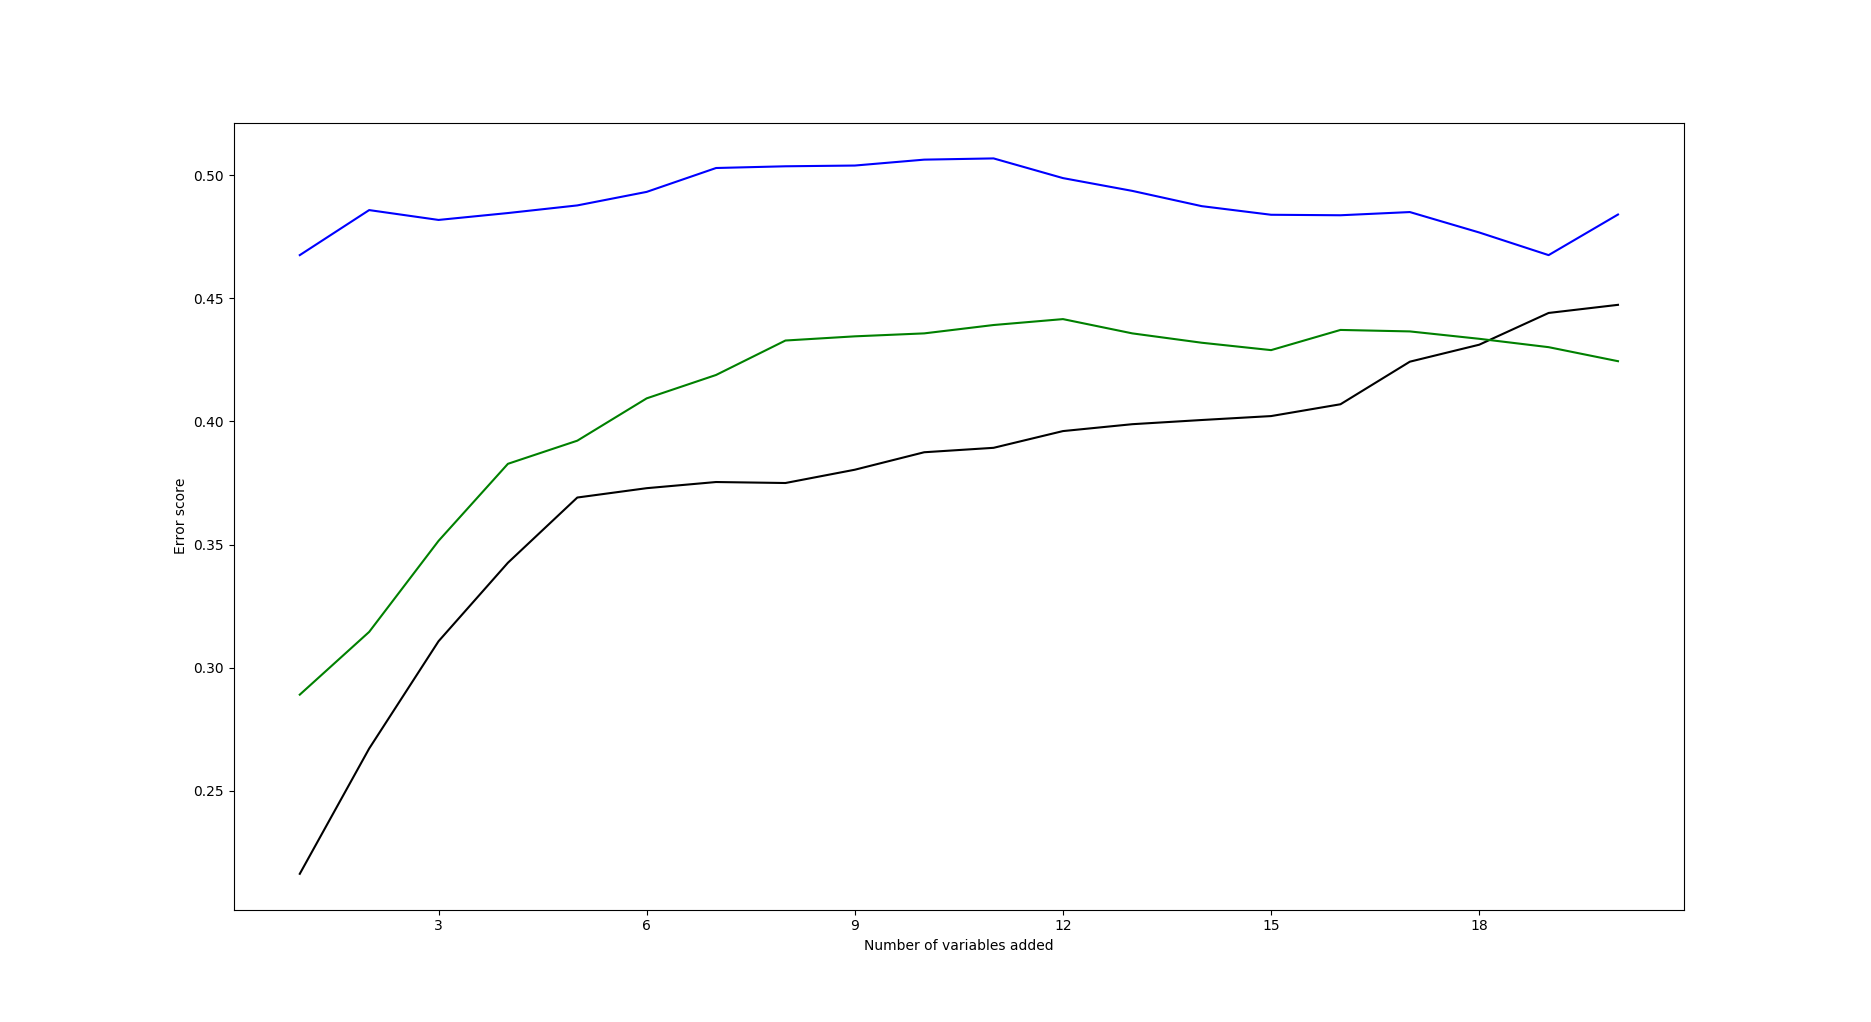
\includegraphics[scale=0.4]{example}\end{center}\caption{Black - Poisson\\Green - Least Squares\\Blue - Least Absolute Deviation}\label{fig:f1}
\end{figure}

\pagebreak\subsubsection*{Important features}

Across the three different regression types, we can identify features that are commonly used. Across the three types there are 40 distinct features selected out of 122 total features. Of these 40, 14 are selected more than once.

\begin{center}
\begin{tabular}{c c l}
\hline
Frequently Selected Features & \# times selected &Description \\
\hline
parking&3&Flag for a park and ride\\
near\_medical&3&Medical jobs within walking distance\\
near\_hospitality&3&Hotel and restaurant jobs within walking distance\\
near\_business&3&Business jobs within walking distance\\
15net\_university&3&university jobs with 15 min transit ride\\
30net\_hunits\_large&3&Housing units in buildings of over 20 units within 30 min ride\\
near\_population&2&Total number of people within walking distance\\
near\_labor\_force&2&People older than 16, employed or looking for a job within walking\\
near\_hunits\_vacant&2&Unoccupied housing units within walking distance\\
near\_finance&2&Jobs in finance within walking distance\\
near\_entertainment&2&Jobs in entertainment within walking distance\\
15net\_hunits\_old&2&Housing units built before 1940 within 15 minute transit ride\\
15net\_hospitality&2&Hotel and restaurant jobs within 15 minute transit ride \\
30net\_university&2&University jobs within 30 minute transit ride\\
\end{tabular}
\end{center}

An interesting note is that of the selected features, there are 30 walking distance features, 14 15 minute ride features, 9 30 minute ride features, and only 4 60 minute ride features. Of those 4 60 minute ride features, none are used by more than one of the regression types. The Atlanta system is small enough that that every station is within 60 minute of any other. Of the remaining systems, only LA and Chicago are really large enough for the 60 minute features to be significantly different from each other. Since the majority of the jobs and people are in the downtown and the downtown is well under 60 minutes from any station, most of hte 60 minute features are very similar to each other. For the LAD regression, this causes a lot of problems with convergence, with a constant feature for an intercept an another near-constant feature. I think that for future analyses, I will drop the 60 minute features. 

\end{document}